\documentclass[aspectratio=169]{beamer}
\usetheme{Madrid}
\usecolortheme{default}

\usepackage{fontspec}
\usepackage{polyglossia}
\setmainlanguage{spanish}
\usepackage{graphicx}
\usepackage{amsmath}
\usepackage{booktabs}
\usepackage{xcolor}

\definecolor{usalred}{RGB}{140,21,21}
\definecolor{usalreddark}{RGB}{80,10,10}
\usecolortheme[named=usalred]{structure}
\setbeamercolor{title}{bg=usalred,fg=white}
\setbeamercolor{frametitle}{bg=usalred,fg=white}
\setbeamercolor{palette primary}{bg=usalred,fg=white}
\setbeamercolor{palette secondary}{bg=usalreddark,fg=white}
\setbeamercolor{palette tertiary}{bg=usalreddark,fg=white}
\setbeamercolor{palette quaternary}{bg=usalred,fg=white}
\setbeamercolor{block title}{bg=usalred,fg=white}
\setbeamercolor{section in toc}{fg=usalred}

\setbeamertemplate{navigation symbols}{}
\setbeamerfont{footnote}{size=\tiny}

\setbeamercolor{footlinebox}{bg=usalreddark,fg=white}
\setbeamertemplate{footline}{
  \leavevmode
  \hbox{%
  \begin{beamercolorbox}[wd=.55\paperwidth,ht=2.6ex,dp=1.2ex,left,leftskip=1em]{footlinebox}
    \usebeamerfont{footline}\tiny Fundamentos e introducción al aprendizaje automático --- Cap. 3
  \end{beamercolorbox}%
  \begin{beamercolorbox}[wd=.32\paperwidth,ht=2.6ex,dp=1.2ex,center]{footlinebox}
    \usebeamerfont{footline}\tiny \insertsectionhead
  \end{beamercolorbox}%
  \begin{beamercolorbox}[wd=.13\paperwidth,ht=2.6ex,dp=1.2ex,right,rightskip=1em]{footlinebox}
    \usebeamerfont{footline}\tiny \insertframenumber{}/\inserttotalframenumber
  \end{beamercolorbox}%
  }
}

\newcommand{\fuente}[1]{{\footnotesize\textit{Fuente: #1}}}
\newcommand{\ejemplo}[1]{\par\vspace{0.4em}{\small\color{usalreddark}\textbf{Ejemplo:} #1}}

\title[3. Aprendizaje No Supervisado]{Capítulo 3: Aprendizaje\\No Supervisado}
\author{Universidad de Salamanca}
\institute{Facultad de Ciencias}
\date{Programación Avanzada}

\AtBeginSection[]{
  \begin{frame}{Contenidos}
    \tableofcontents[currentsection]
  \end{frame}
}

\newcommand{\titleslide}{%
\begin{frame}
  \titlepage
  \vspace{-0.5em}
  {\footnotesize Diego M. Jiménez-Bravo \quad$\cdot$\quad \texttt{dmjimenez@usal.es}}
\end{frame}
}

\begin{document}

\titleslide

\begin{frame}{Índice}
  \tableofcontents
\end{frame}

% ============================================================
\section{Introducción}

\begin{frame}{¿Qué es el aprendizaje no supervisado?}
  \small
  A diferencia de los capítulos anteriores, aquí el entrenamiento \textbf{no está guiado} por ninguna etiqueta o variable objetivo. El sistema no recibe un criterio de ``verdad fundamental'' (\textit{ground-truth}); en su lugar, debe explorar las relaciones matemáticas intrínsecas de los datos para revelar su estructura oculta.

  Técnicamente, mientras el aprendizaje supervisado busca aproximar la relación $X \rightarrow y$, el no supervisado trabaja ``a ciegas'' para descubrir la \textbf{estructura latente} de los propios datos $X$, sin ninguna respuesta correcta de referencia.

  Como ilustró el científico Yann LeCun: \textit{``Si la inteligencia fuera un pastel, el aprendizaje no supervisado sería el bizcocho, el supervisado sería la cobertura, y el aprendizaje por refuerzo sería la cereza''}. La inmensa mayoría de los datos del mundo real no vienen etiquetados, lo que hace de este paradigma un pilar fundamental del aprendizaje automático.

  Existen tres grandes familias de técnicas: \textbf{\textit{clustering}} (agrupar datos similares), \textbf{reducción de dimensionalidad} (simplificar datos complejos) y \textbf{detección de anomalías} (identificar casos raros).
\end{frame}

\begin{frame}{Aplicaciones prácticas}
  \small
  \begin{itemize}
    \item \textbf{Segmentación de mercado}: agrupar clientes en nichos homogéneos según sus datos demográficos y de consumo, sin definir las categorías de antemano, para dirigir campañas específicas.
    \item \textbf{Visualización de datos complejos}: proyectar conjuntos de datos con cientos de variables a representaciones en 2D o 3D, preservando su estructura, para que una persona pueda entenderlos de un vistazo.
    \item \textbf{Sistemas de recomendación}: agrupar usuarios con gustos afines o productos con características similares para predecir preferencias implícitas.
    \item \textbf{Detección de anomalías}: modelar el comportamiento ``normal'' de los datos para identificar automáticamente fraudes financieros o fallos en líneas de fabricación.
  \end{itemize}
  \ejemplo{una tienda online que agrupa a sus clientes por hábitos de compra (sin decirle previamente qué grupos buscar) para después diseñar ofertas distintas para cada grupo --- eso es \textit{clustering} aplicado a segmentación de mercado.}
\end{frame}

% ============================================================
\section{3.1 Clustering}

\begin{frame}{¿Qué es el \textit{clustering}?}
  El \textit{clustering} (o agrupamiento) es la técnica más extendida del aprendizaje no supervisado. Su objetivo es \textbf{particionar} un conjunto de datos en subgrupos cuyos miembros compartan una \textbf{alta similitud interna} y, al mismo tiempo, presenten una \textbf{alta diferenciación} respecto a los miembros de otros subgrupos.

  Existen distintas familias de algoritmos, según cómo definan la pertenencia a un grupo: basados en \textbf{centroides} ($K$-\textit{means}), basados en \textbf{jerarquías} (\textit{clustering} jerárquico) y basados en \textbf{densidad} (DBSCAN). Los estudiaremos uno por uno.
\end{frame}

\begin{frame}{$K$-\textit{means}: mecánica del algoritmo}
  \small
  El $K$-\textit{means} es un algoritmo de agrupación basado en \textbf{centroides}: busca particionar un conjunto de observaciones en $K$ \textit{clusters} distintos, donde cada centroide actúa como el ``centro de gravedad'' de su grupo. Su meta matemática es minimizar la \textbf{inercia intracluster} (WCSS, \textit{Within-cluster Sum of Squares}). El proceso se repite iterativamente:
  \begin{enumerate}
    \item \textbf{Inicialización}: se eligen $K$ puntos aleatorios como centroides iniciales.
    \item \textbf{Asignación}: cada muestra se une al centroide más cercano (normalmente, por distancia euclídea).
    \item \textbf{Actualización}: cada centroide se recalcula como la media de todas las muestras asignadas a su grupo.
    \item Se repiten los pasos 2 y 3 hasta que los centroides dejan de moverse: la \textbf{convergencia}.
  \end{enumerate}
  \begin{center}
    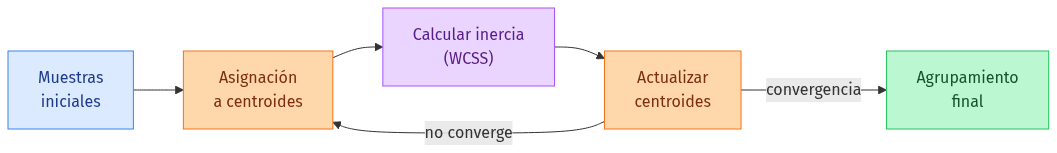
\includegraphics[width=0.42\textwidth]{../book/_static/generated/diagrams_pdf/es/02_aprendizaje_no_supervisado_01_clustering_01.png}
  \end{center}
\end{frame}

\begin{frame}{$K$-\textit{means}: proceso visual}
  La siguiente figura muestra las tres etapas sobre un conjunto de datos con tres grupos naturales: los centroides (marcados con X) parten de posiciones aleatorias y convergen hacia el centro de cada grupo tras pocas iteraciones.
  \begin{center}
    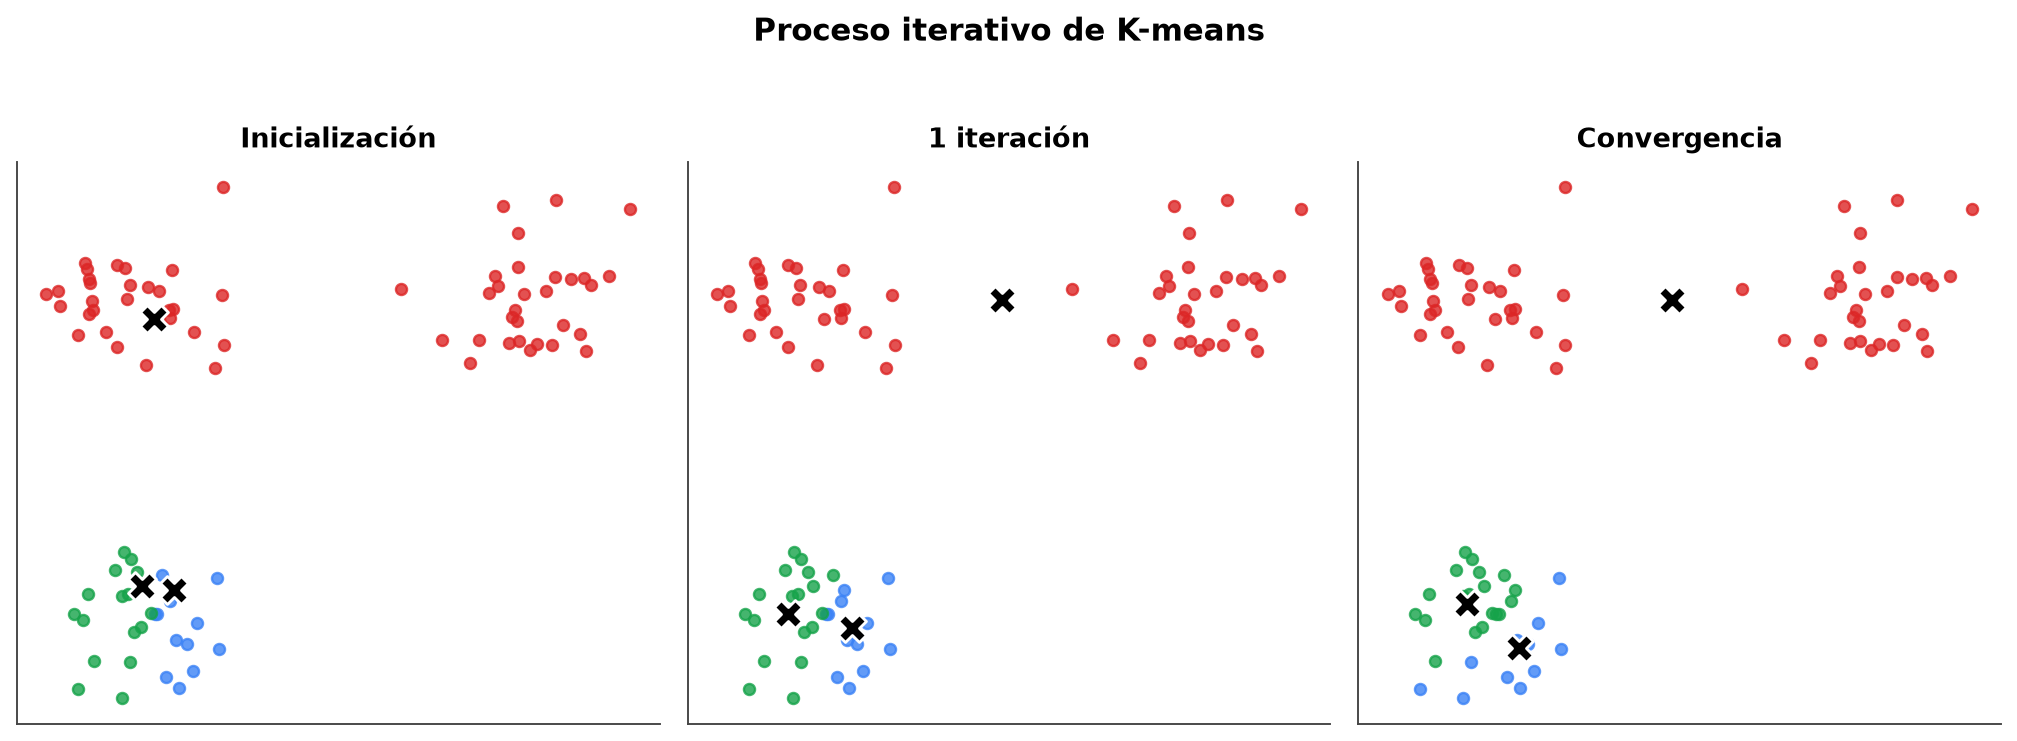
\includegraphics[width=0.8\textwidth]{../book/_static/generated/figures/es/kmeans_process.png}
  \end{center}
  \ejemplo{es como asignar mesas en una fiesta: cada invitado se sienta en la mesa más cercana; luego cada mesa se recoloca al centro de sus invitados; y se repite el proceso hasta que nadie tiene que moverse.}
\end{frame}

\begin{frame}{$K$-\textit{means}++: el problema de la inicialización}
  \small
  El $K$-\textit{means} es un algoritmo \textbf{heurístico} y, por tanto, muy sensible a la inicialización aleatoria de sus centroides. Si los centroides iniciales caen en regiones desfavorables, el algoritmo puede converger en un \textbf{mínimo local subóptimo} --- un agrupamiento que parece bueno localmente pero no es el mejor posible.

  Para mitigar este problema se usa la inicialización \textbf{$K$-\textit{means}++}:
  \begin{itemize}
    \item El primer centroide se elige al azar entre los puntos de datos.
    \item Cada centroide siguiente se elige de forma probabilística, dando más probabilidad a los puntos que están \textbf{más lejos} de los centroides ya elegidos.
  \end{itemize}
  Este ``sembrado inteligente'' asegura que los centroides iniciales queden bien repartidos por el espacio, acelerando la convergencia y mejorando la calidad del resultado final.
\end{frame}

\begin{frame}{El método del codo}
  Como el número de \textit{clusters} $K$ es un hiperparámetro que hay que fijar antes de entrenar, necesitamos un criterio para elegirlo. El \textbf{método del codo} consiste en graficar la inercia (WCSS) frente a distintos valores de $K$:
  \begin{itemize}
    \item A medida que $K$ aumenta, la inercia disminuye de forma natural (los grupos son más pequeños y compactos).
    \item El valor óptimo de $K$ está en el punto donde la curva deja de caer bruscamente y se vuelve casi plana: el ``codo''.
  \end{itemize}
  \begin{center}
    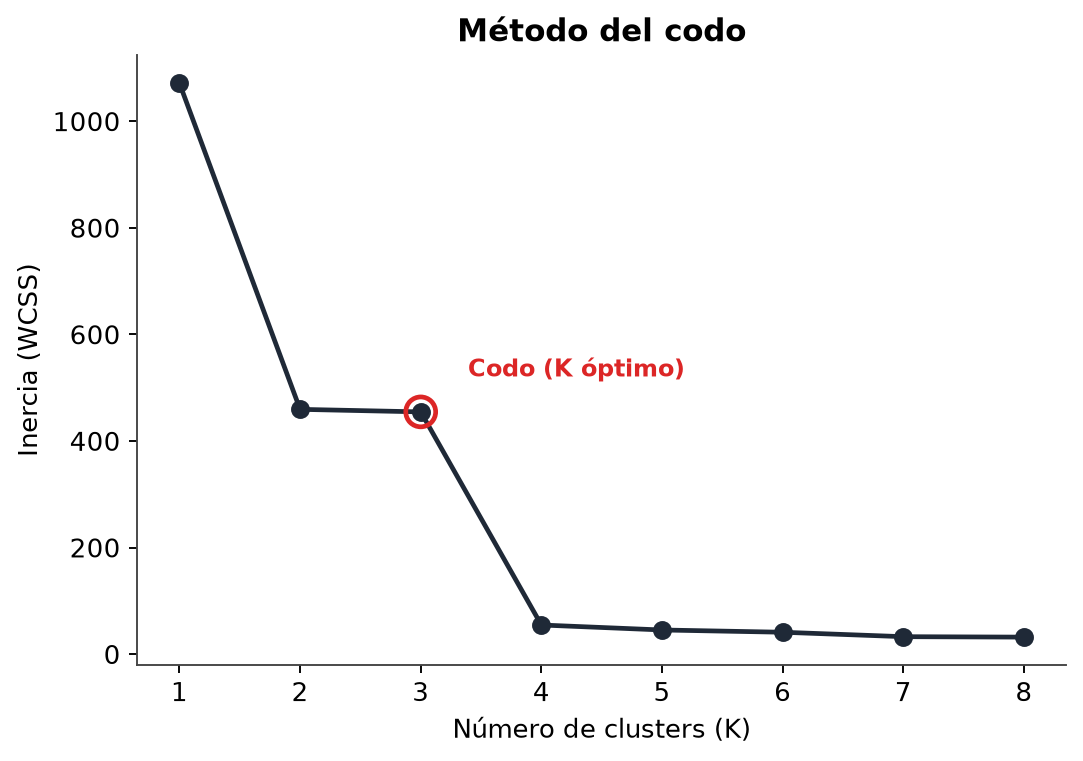
\includegraphics[width=0.38\textwidth]{../book/_static/generated/figures/es/elbow_method.png}
  \end{center}
\end{frame}

\begin{frame}{\textit{Clustering} jerárquico: enfoque aglomerativo}
  \small
  El \textit{clustering} jerárquico agrupa datos \textbf{sin necesidad de fijar} $K$ de antemano, y genera una estructura jerárquica fácil de visualizar. El método más común es el \textbf{aglomerativo} (de abajo a arriba):
  \begin{enumerate}
    \item Se empieza tratando cada observación individual como su propio \textit{cluster}.
    \item En cada paso, se calculan las distancias entre todos los \textit{clusters} y se \textbf{fusionan los dos más cercanos}.
    \item El proceso se repite hasta que todas las muestras quedan integradas en un único \textit{cluster} global.
  \end{enumerate}
\end{frame}

\begin{frame}{Dendrogramas e interpretación de cortes}
  La jerarquía de fusiones se representa gráficamente mediante un \textbf{dendrograma}: un diagrama de árbol donde el eje vertical indica la distancia (o disimilitud) a la que se fusionó cada par de grupos.

  El usuario puede elegir el número final de \textit{clusters} haciendo un \textbf{corte horizontal} a una altura concreta: el número de líneas que atraviesa el corte es el número de grupos resultantes. Esto ofrece una flexibilidad que algoritmos rígidos como $K$-\textit{means} no tienen.
  \begin{center}
    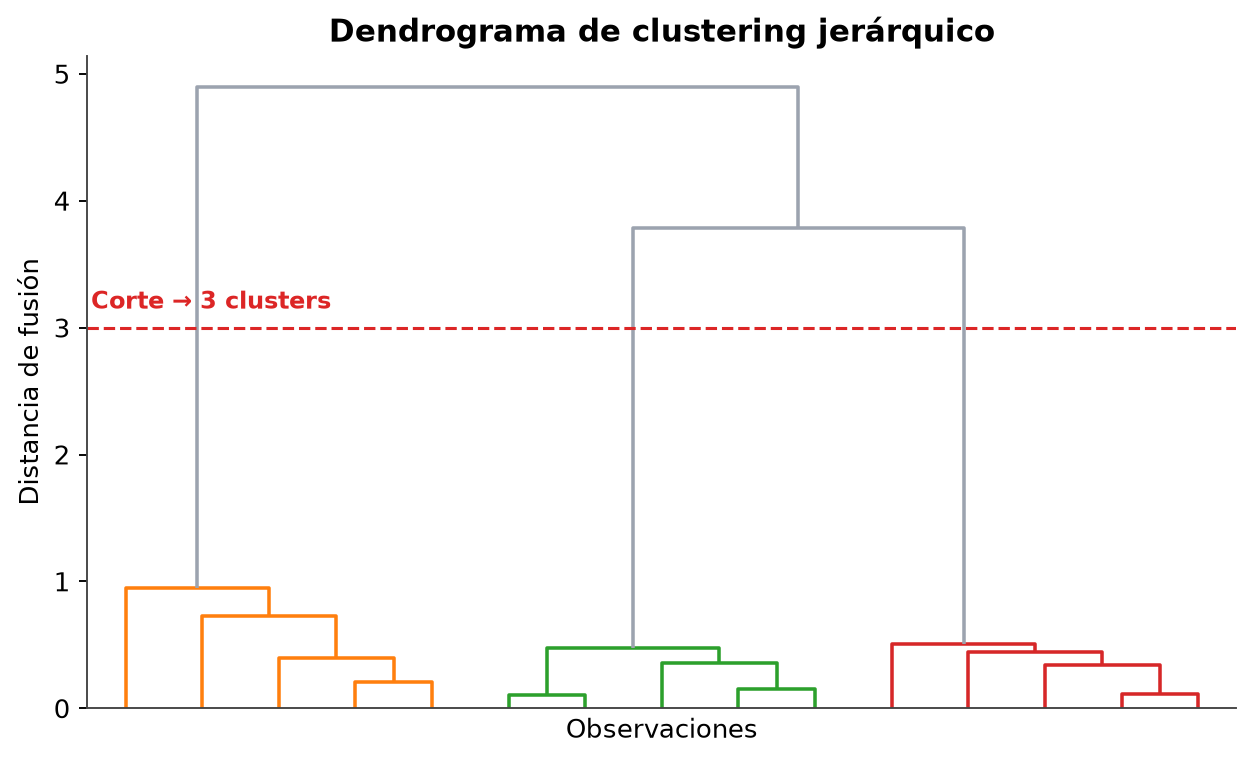
\includegraphics[width=0.48\textwidth]{../book/_static/generated/figures/es/dendrogram.png}
  \end{center}
\end{frame}

\begin{frame}{Criterios de enlace (\textit{linkage})}
  \small
  Para decidir qué \textit{clusters} fusionar en cada paso, hace falta definir cómo medir la distancia entre grupos (no entre puntos individuales):
  \begin{itemize}
    \item \textbf{Enlace completo}: la distancia \textbf{máxima} entre cualquier par de puntos de los dos grupos. Produce \textit{clusters} compactos y bien balanceados.
    \item \textbf{Enlace simple}: la distancia \textbf{mínima} entre cualquier par. Es sensible al ruido y puede producir un efecto de ``encadenamiento'' (grupos alargados y difusos).
    \item \textbf{Enlace promedio}: el promedio de \textbf{todas} las distancias entre puntos de ambos grupos. Equilibra la estabilidad del enlace completo con la tolerancia del simple.
  \end{itemize}
  \begin{center}
    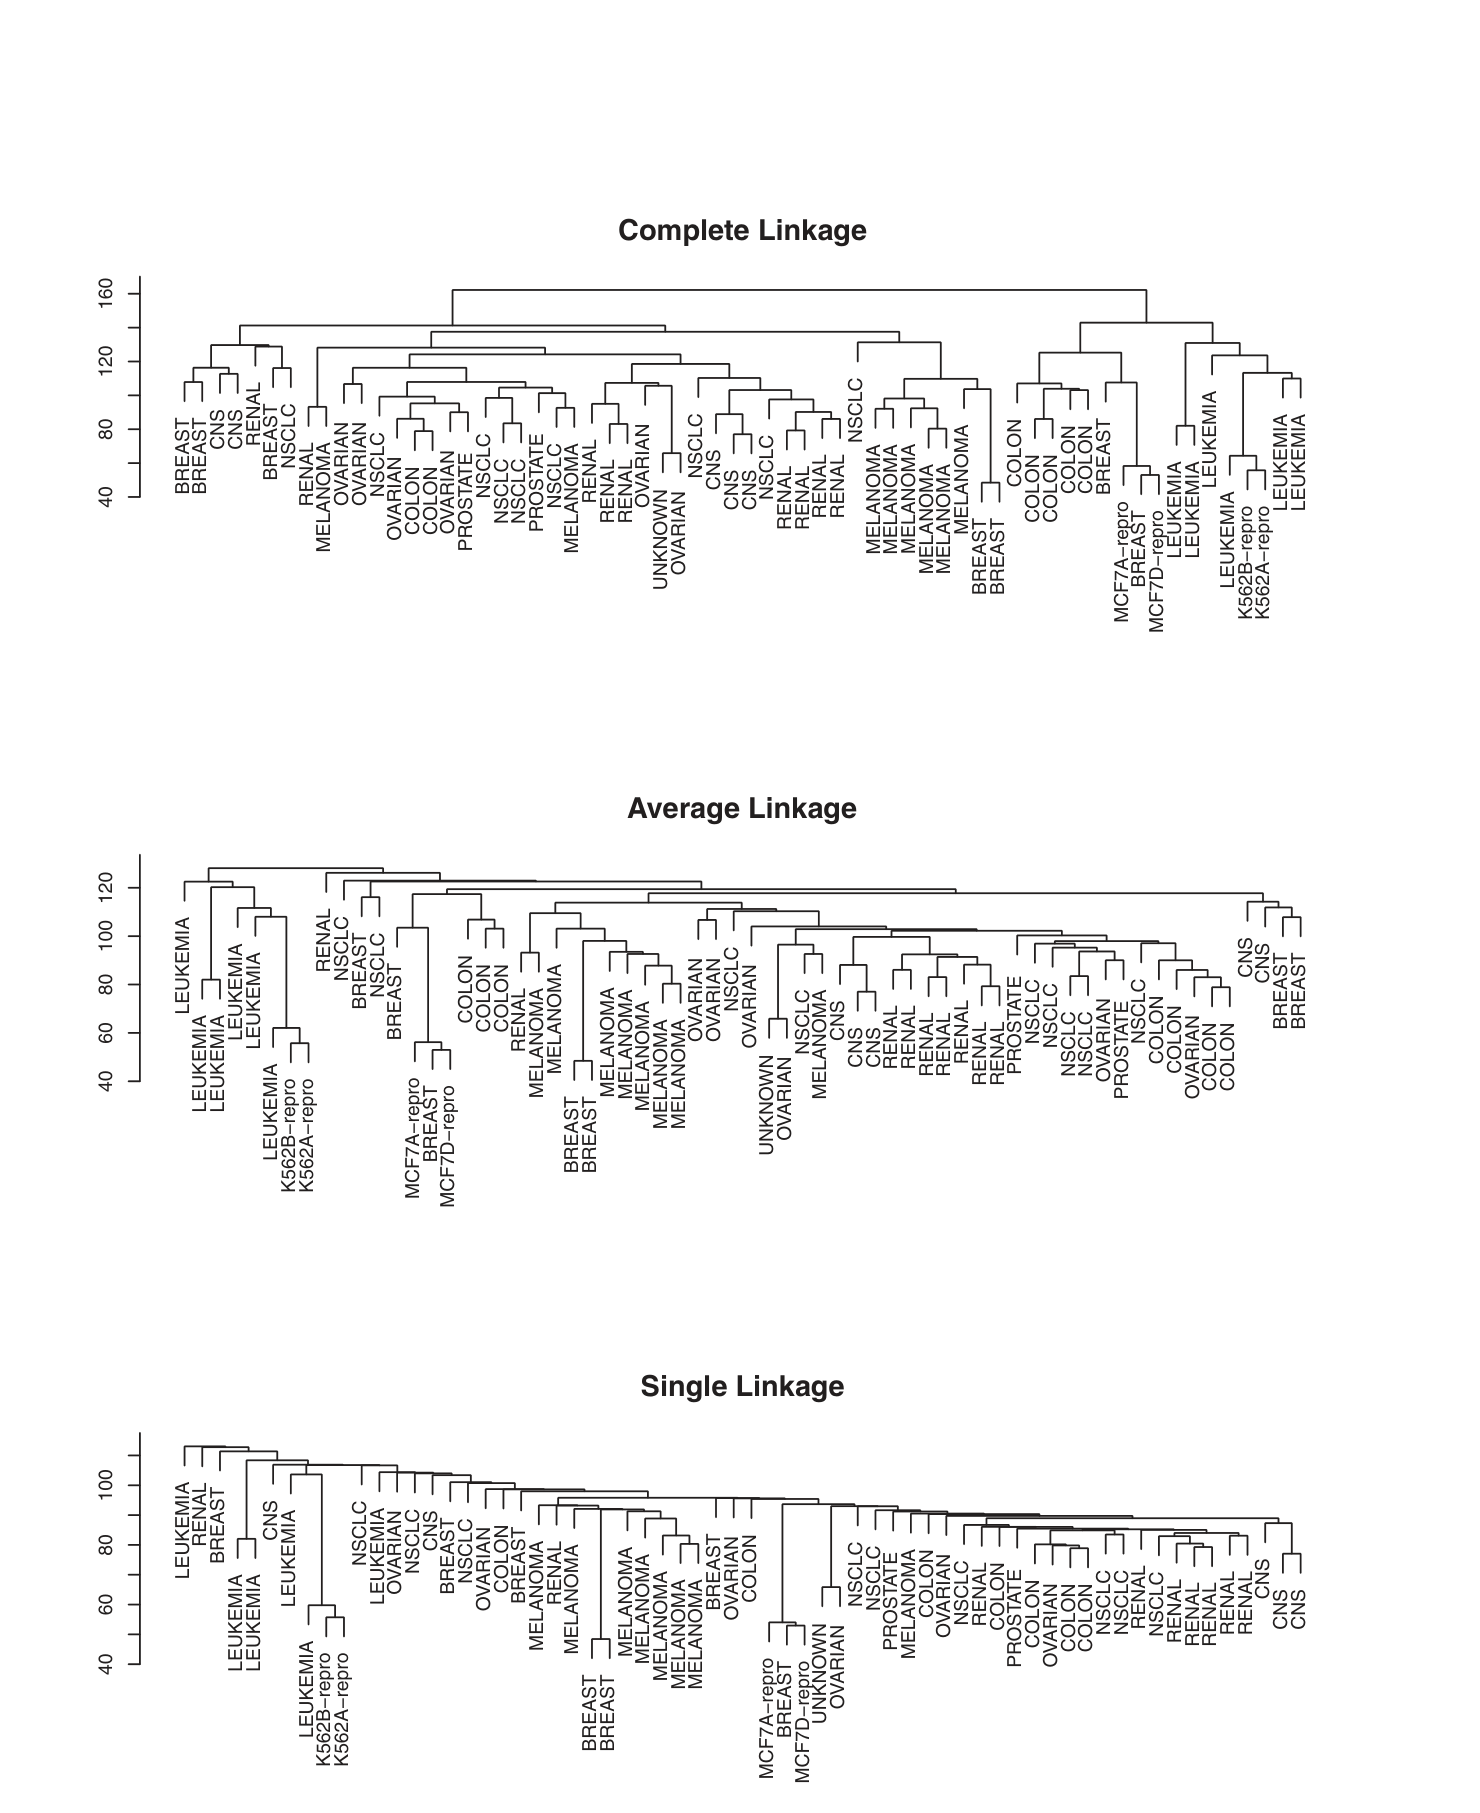
\includegraphics[width=0.17\textwidth]{../book/_static/book_figures/islr_fig10_17_nci60_dendrogram.png}
  \end{center}
  {\footnotesize\fuente{James, Witten, Hastie \& Tibshirani (2013), \textit{An Introduction to Statistical Learning}, Fig. 10.17.}}
\end{frame}

\begin{frame}{DBSCAN: fundamentos y parámetros}
  \small
  El algoritmo \textbf{DBSCAN} (\textit{Density-Based Spatial Clustering of Applications with Noise}) define los grupos según la \textbf{densidad local} de los datos, en vez de por cercanía a un centroide o por jerarquía. Esto le permite descubrir \textit{clusters} de formas geométricas arbitrarias y aislar el ruido de forma natural.

  Requiere dos hiperparámetros:
  \begin{itemize}
    \item \textbf{$\epsilon$ (épsilon)}: el radio de la vecindad alrededor de cualquier punto.
    \item \textbf{MinPts}: el número mínimo de puntos que debe haber dentro de ese radio para considerar la región ``densa''.
  \end{itemize}
\end{frame}

\begin{frame}{DBSCAN: clasificación de puntos}
  Durante su ejecución, DBSCAN clasifica cada punto en una de tres categorías según la densidad de su vecindad:
  \begin{itemize}
    \item \textbf{Puntos núcleo}: su vecindad de radio $\epsilon$ contiene al menos MinPts muestras.
    \item \textbf{Puntos frontera}: no llegan a MinPts por sí mismos, pero están dentro de la vecindad de un punto núcleo.
    \item \textbf{Puntos de ruido}: no son ni núcleo ni frontera --- se consideran anomalías y no se asignan a ningún \textit{cluster}.
  \end{itemize}
  \begin{center}
    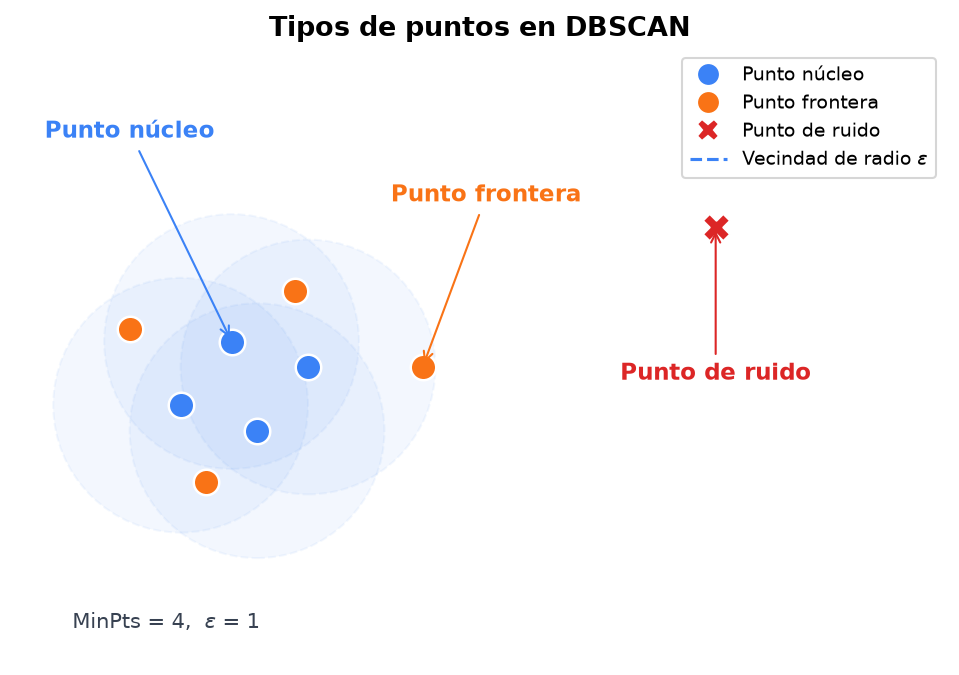
\includegraphics[width=0.38\textwidth]{../book/_static/generated/figures/es/dbscan_point_types.png}
  \end{center}
\end{frame}

\begin{frame}{DBSCAN: ventajas frente a $K$-\textit{means}}
  \small
  \begin{itemize}
    \item \textbf{Robustez ante el ruido}: $K$-\textit{means} obliga a cada muestra a pertenecer a un \textit{cluster} (desplazando artificialmente los centroides ante valores atípicos); DBSCAN identifica y aísla el ruido de forma nativa.
    \item \textbf{Flexibilidad geométrica}: no asume que los \textit{clusters} deban ser esféricos, por lo que puede descubrir formas alargadas, anidadas o irregulares.
  \end{itemize}
  \begin{center}
    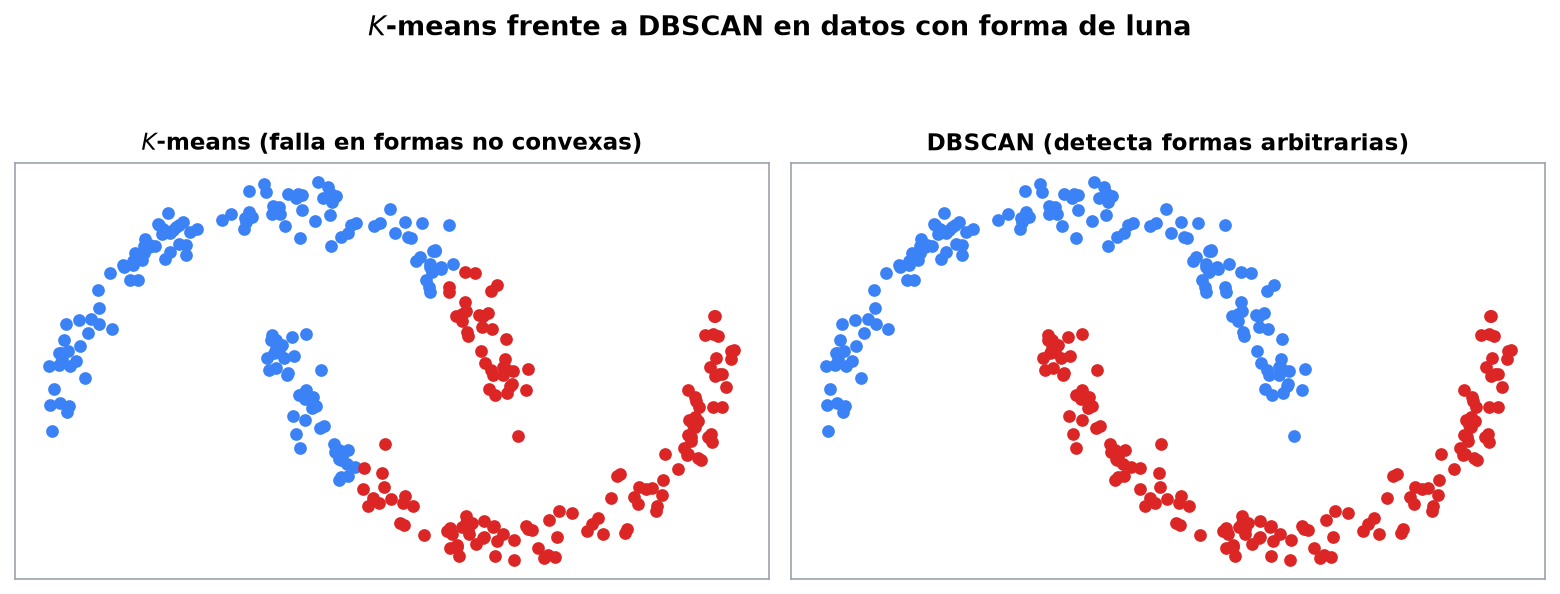
\includegraphics[width=0.62\textwidth]{../book/_static/generated/figures/es/dbscan_vs_kmeans.png}
  \end{center}
\end{frame}

\begin{frame}{Evaluación: el coeficiente de silueta}
  \small
  Sin etiquetas, ¿cómo sabemos si un \textit{clustering} es bueno? El \textbf{coeficiente de silueta} compara, para cada punto, lo cerca que está de su propio grupo frente a lo cerca que está del grupo vecino más próximo:
  \[ sc(i) = \frac{b_i - a_i}{\max(a_i, b_i)} \]
  El valor va de $-1$ a $1$: cerca de $+1$ indica un punto bien agrupado y alejado de otros \textit{clusters}; cerca de $0$, un punto en la frontera entre dos grupos; y negativo sugiere que el punto está mal asignado.
  \begin{center}
    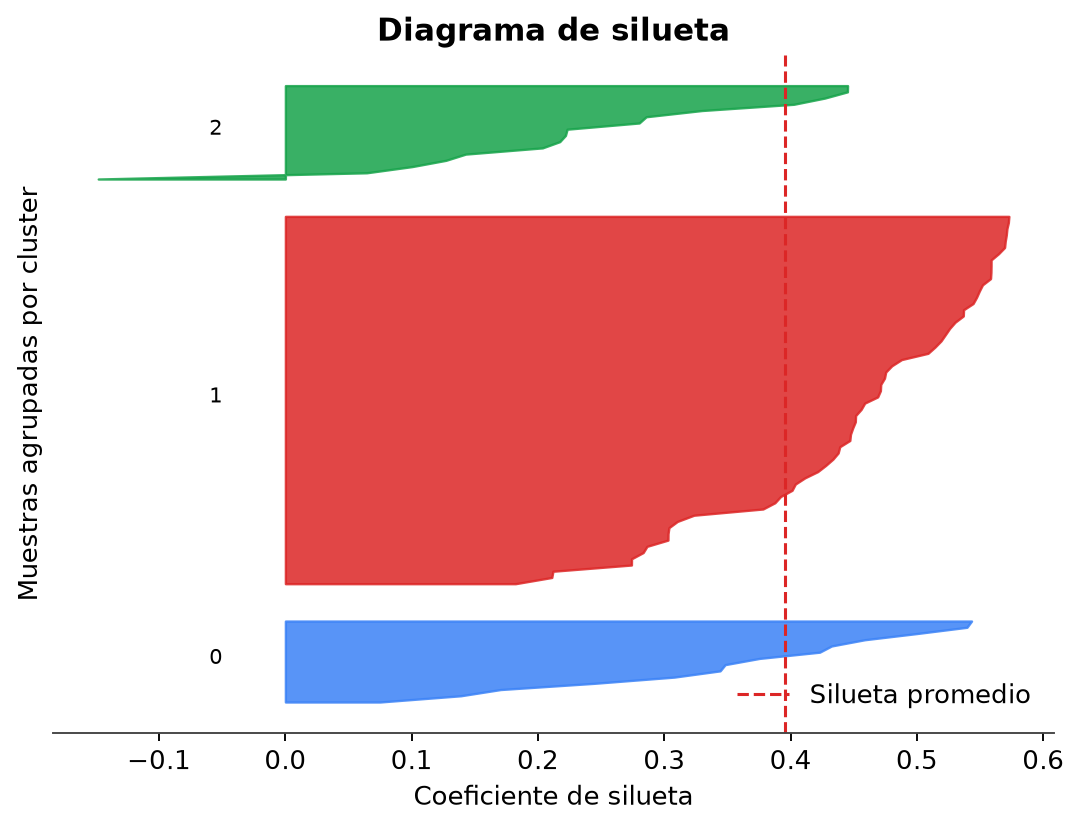
\includegraphics[width=0.3\textwidth]{../book/_static/generated/figures/es/silhouette_diagram.png}
  \end{center}
\end{frame}

\begin{frame}{Evaluación: el estadístico \textit{gap}}
  \small
  El \textbf{estadístico \textit{gap}} es otra forma de elegir el número óptimo de \textit{clusters}, más rigurosa que el método del codo: compara la inercia observada en los datos reales con la que se esperaría si los datos no tuvieran ninguna estructura de agrupamiento.

  Su gran ventaja: puede detectar cuándo la respuesta correcta es que \textbf{no hay ningún agrupamiento real} en los datos --- algo que el método del codo o la silueta no siempre dejan claro.
\end{frame}

\begin{frame}{Otros criterios de evaluación}
  \small
  Existen más formas de evaluar un \textit{clustering}, sobre todo cuando se usan modelos probabilísticos:
  \begin{itemize}
    \item \textbf{AIC y BIC}: comparan modelos penalizando los que tienen demasiados parámetros, para no quedarnos siempre con el más complejo.
    \item \textbf{Correlación cofenética}: comprueba si un dendrograma refleja bien las distancias reales entre los datos.
  \end{itemize}
  En la práctica, estos criterios rara vez se calculan a mano: las librerías de \textit{machine learning} los aplican automáticamente para comparar modelos.
\end{frame}

\begin{frame}{Evaluación externa con datos etiquetados}
  \small
  Cuando sí disponemos de etiquetas de referencia (aunque no se hayan usado para entrenar), podemos comprobar qué tan bien encajan los grupos descubiertos con las categorías reales:
  \begin{itemize}
    \item \textbf{Pureza}: a cada \textit{cluster} se le asigna la etiqueta más frecuente en su interior, y se mide la proporción de aciertos así obtenida. Su punto débil: no penaliza tener demasiados \textit{clusters} pequeños.
    \item \textbf{Índice Rand ajustado (ARI)}: compara si el modelo agrupó las muestras de forma parecida a como lo harían las clases reales, corrigiendo el resultado que se obtendría por puro azar.
  \end{itemize}
\end{frame}

% ============================================================
\section{3.2 Reducción de dimensionalidad}

\begin{frame}{La maldición de la dimensionalidad}
  \small
  En la analítica moderna es habitual encontrar conjuntos de datos con cientos o miles de variables. Trabajar directamente en esos espacios de alta dimensión tiene graves inconvenientes, conocidos como la \textbf{maldición de la dimensionalidad}: a medida que aumenta el número de dimensiones, el volumen del espacio crece exponencialmente, y cualquier conjunto de datos real ---por grande que sea--- lo puebla de forma extremadamente \textbf{dispersa}. Las muestras dejan de tener ``vecinos'' cercanos de verdad, y las distancias entre puntos se vuelven casi indistinguibles.
  \begin{center}
    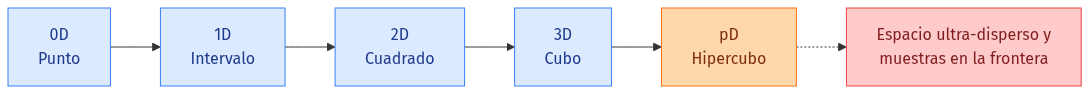
\includegraphics[width=0.7\textwidth]{../book/_static/generated/diagrams_pdf/es/02_aprendizaje_no_supervisado_02_reduccion_dimensionalidad_01.png}
  \end{center}
\end{frame}

\begin{frame}{¿Por qué reducir dimensiones?}
  La reducción de dimensionalidad aborda este problema proyectando o comprimiendo los datos en un espacio de baja dimensión (habitualmente 2D o 3D). Esto ofrece varias ventajas:
  \begin{itemize}
    \item Acelera drásticamente la computación posterior.
    \item Mitiga el riesgo de \textit{overfitting}.
    \item Es indispensable para \textbf{visualizar} datos complejos y para extraer factores latentes explicables.
  \end{itemize}
  \begin{center}
    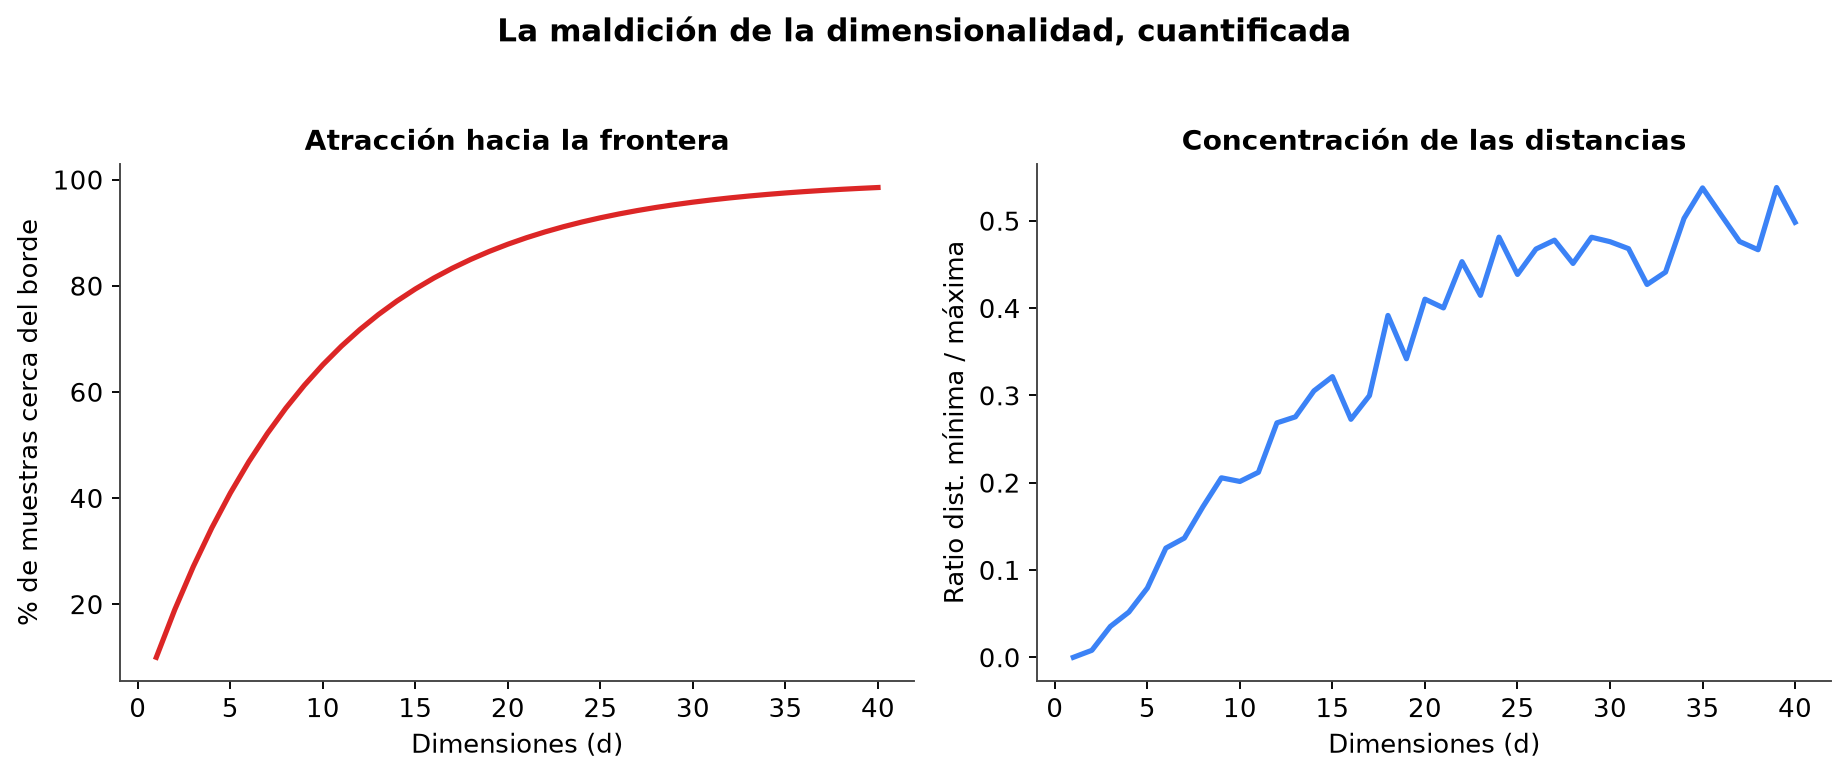
\includegraphics[width=0.6\textwidth]{../book/_static/generated/figures/es/curse_of_dimensionality.png}
  \end{center}
\end{frame}

\begin{frame}{PCA: la dirección de máxima varianza}
  \small
  El \textbf{Análisis de Componentes Principales} (PCA) es el algoritmo de reducción de dimensionalidad lineal por excelencia. Proyecta ortogonalmente los datos originales sobre un subespacio de menor dimensión, minimizando la pérdida de información.

  La \textbf{primera componente principal} (PC1) es la dirección del espacio de características a lo largo de la cual los datos \textbf{varían más}. Al proyectar los datos sobre este eje, se conserva el mayor porcentaje posible de la información original. La \textbf{segunda componente} (PC2) busca la dirección que explica la mayor varianza \textit{restante}, con la condición de ser ortogonal a la primera.
  \begin{center}
    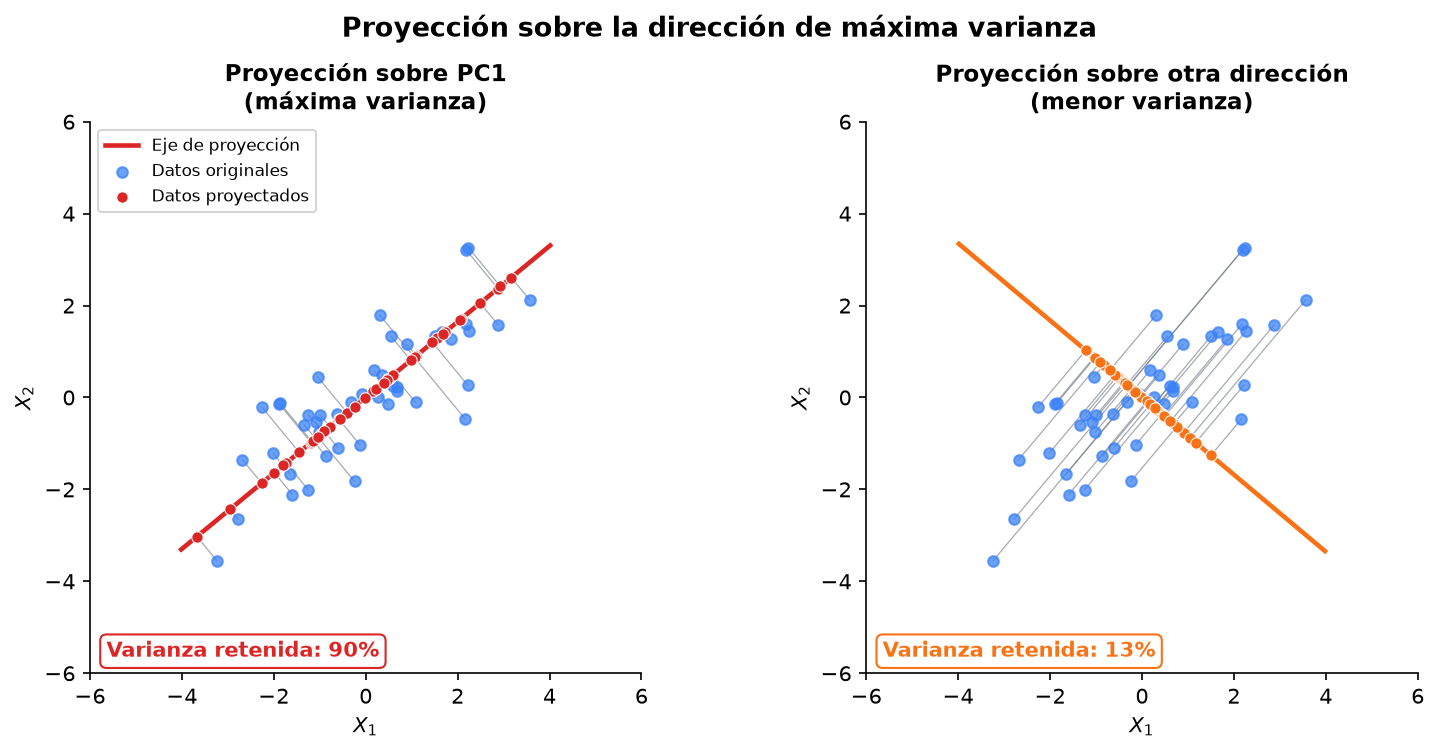
\includegraphics[width=0.5\textwidth]{../book/_static/generated/figures/es/pca_max_variance_projection.png}
  \end{center}
\end{frame}

\begin{frame}{PCA: direcciones principales y reconstrucción}
  \small
  PCA puede entenderse como un algoritmo de compresión: un ``codificador'' reduce cada muestra a una representación más pequeña (sus componentes principales), y un ``decodificador'' la reconstruye de vuelta al espacio original con el mínimo error posible. Cuantas menos componentes se conserven, mayor es la compresión, pero también mayor la información que se pierde.
  \begin{center}
    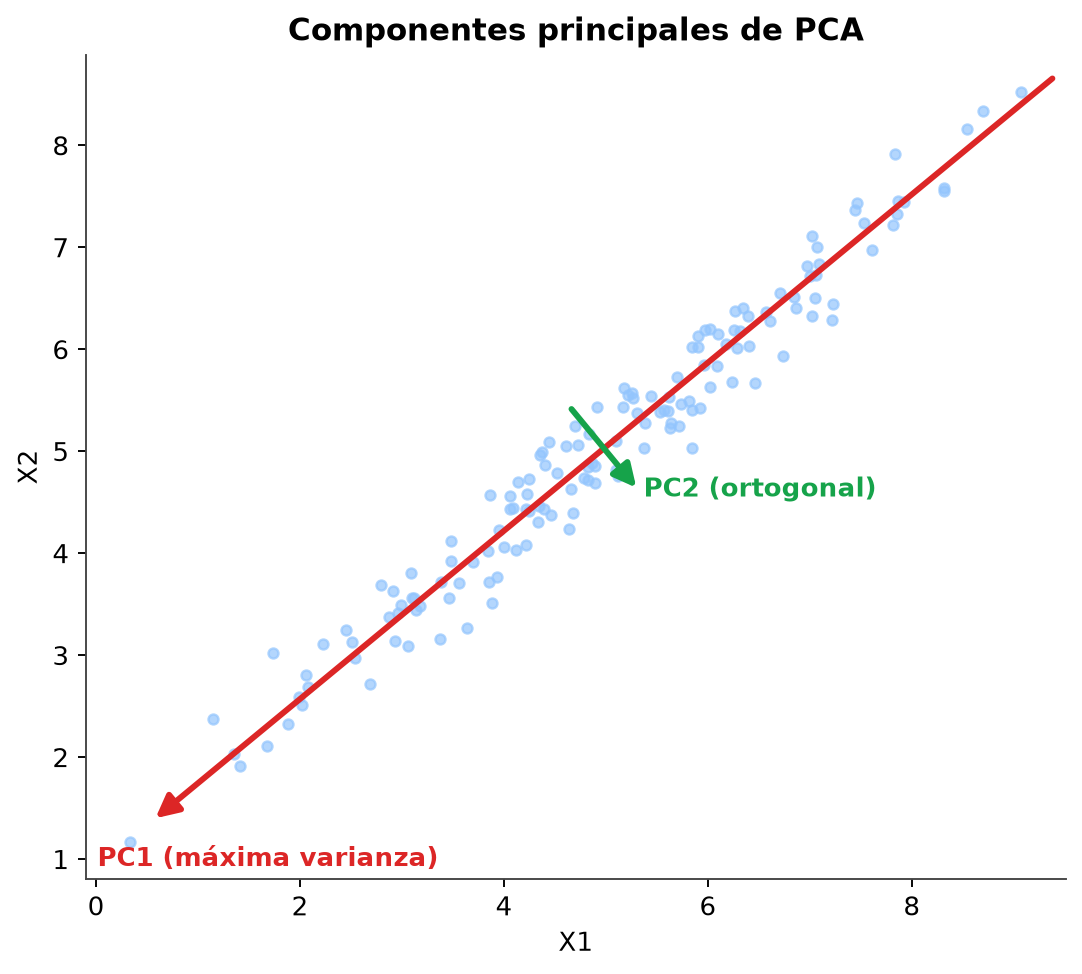
\includegraphics[width=0.32\textwidth]{../book/_static/generated/figures/es/pca_projection.png}
  \end{center}
\end{frame}

\begin{frame}{PCA en datos reales: NCI60 (6830 genes)}
  Un ejemplo real de la utilidad de PCA aparece en el conjunto de datos \textit{NCI60}, donde cada muestra tiene 6830 genes (dimensiones). Al proyectar estas muestras sobre sus tres primeras componentes principales, las líneas celulares del mismo tipo de cáncer (mismo color) tienden a agruparse, pese a la enorme dimensionalidad original.
  \begin{center}
    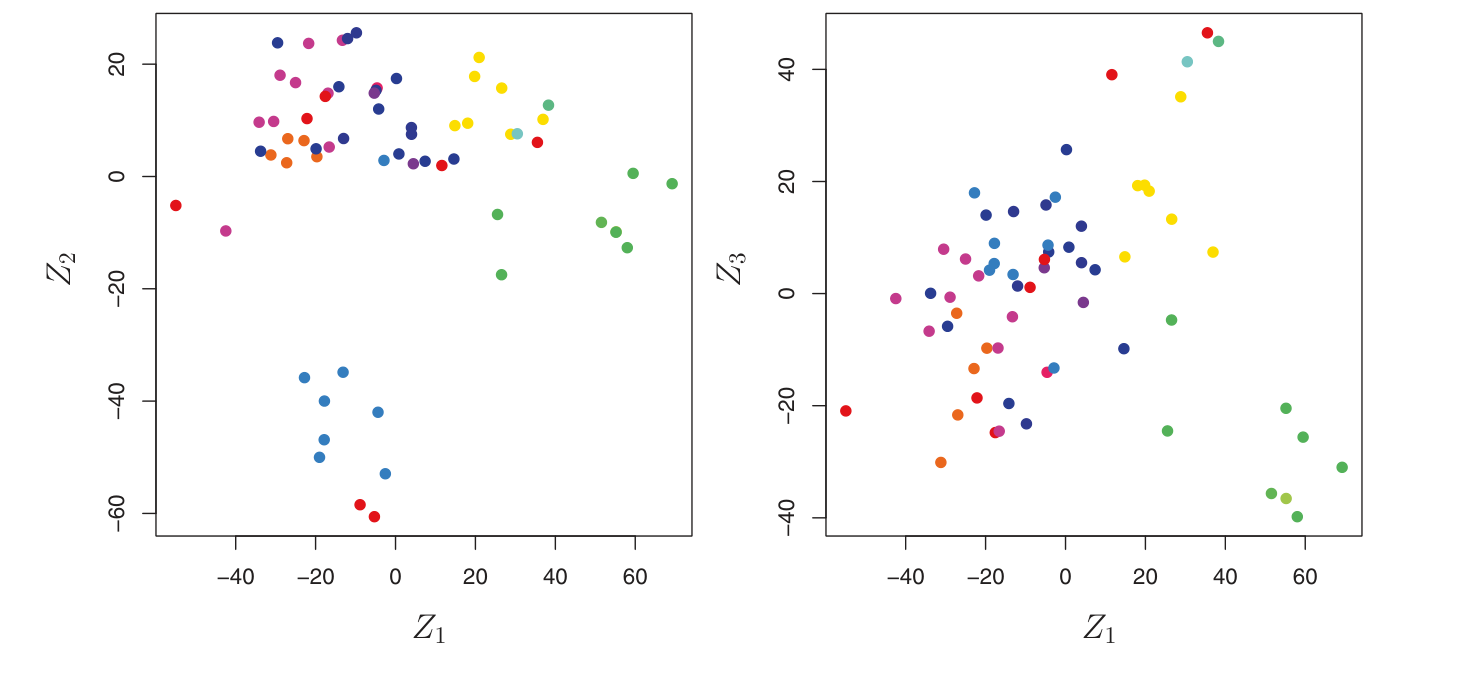
\includegraphics[width=0.55\textwidth]{../book/_static/book_figures/islr_fig10_15_nci60_pca.png}
  \end{center}
  \fuente{James, Witten, Hastie \& Tibshirani (2013), \textit{An Introduction to Statistical Learning}, Fig. 10.15.}
\end{frame}

\begin{frame}{\textit{Manifold learning}: cuando los datos no son planos}
  \small
  PCA es rápido y robusto, pero asume que la estructura interesante de los datos es \textbf{lineal}. Cuando las relaciones son intrínsecamente no lineales (como en el clásico ejemplo del \textit{Swiss roll}, un rollo de papel curvado en 3D), la proyección lineal de PCA colapsa puntos distantes entre sí.

  La \textbf{hipótesis de la variedad} (\textit{manifold hypothesis}) asume que los datos reales (imágenes, voces, textos) viven en una superficie curva de baja dimensión (una \textbf{variedad}), embebida dentro del espacio original de alta dimensión.
  \begin{center}
    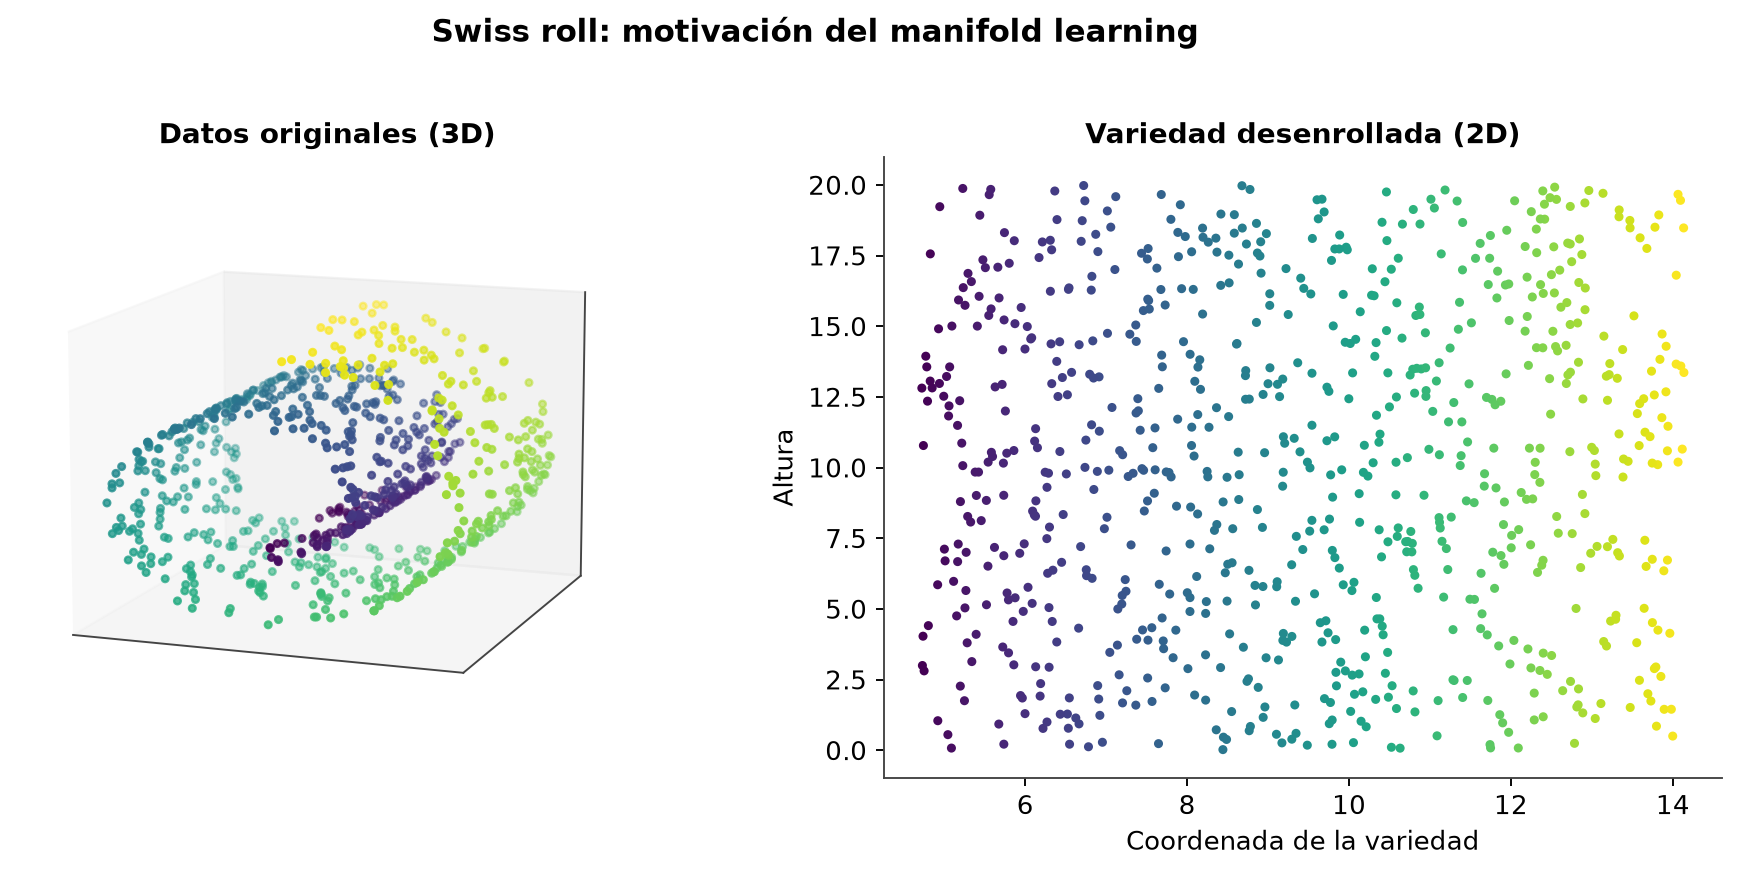
\includegraphics[width=0.54\textwidth]{../book/_static/generated/figures/es/swiss_roll_manifold.png}
  \end{center}
\end{frame}

\begin{frame}{\textit{Kernel} PCA: el truco del \textit{kernel}}
  Para extender PCA a problemas no lineales, \textbf{\textit{kernel} PCA} mapea implícitamente los datos de entrada a un espacio de dimensiones mucho más altas, donde relaciones que eran no lineales en el espacio original se vuelven \textbf{linealmente separables}.

  El siguiente ejemplo clásico lo ilustra: dos clases en círculos concéntricos (izquierda) son imposibles de separar con una línea recta en 2D; tras aplicar el mapeo, quedan a alturas distintas y un simple plano las separa perfectamente.
  \begin{center}
    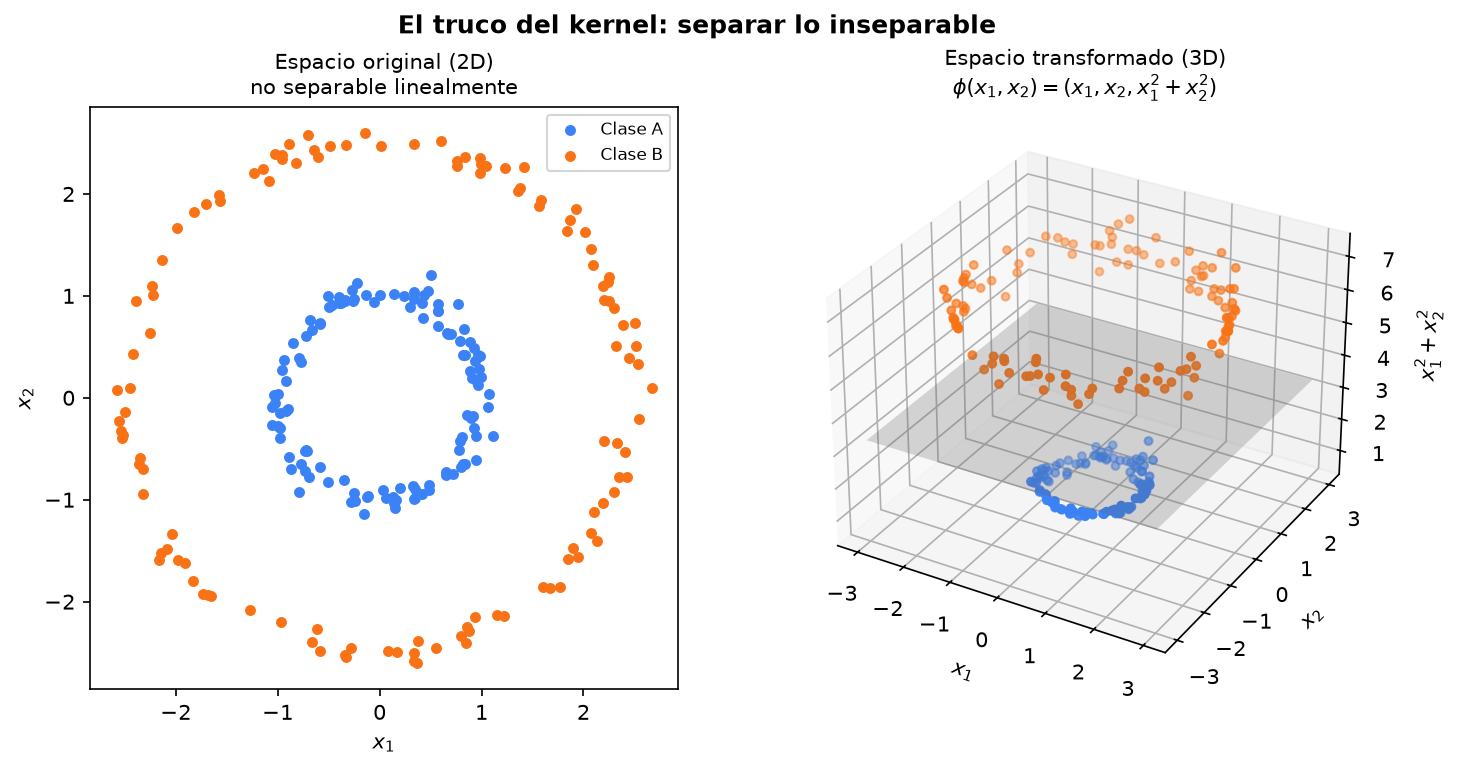
\includegraphics[width=0.5\textwidth]{../book/_static/generated/figures/es/kernel_pca_trick.png}
  \end{center}
\end{frame}

\begin{frame}{$t$-SNE: preservar vecindades locales}
  \small
  Propuesto por Maaten y Hinton (2008), $t$-SNE convierte las distancias entre muestras en \textbf{probabilidades de vecindad}: los puntos cercanos deben seguir cerca tras la proyección a 2D, y los lejanos, lejos. Es la técnica preferida para la \textbf{visualización cualitativa} de agrupamientos complejos, aunque resulta lenta en conjuntos de datos muy grandes.
  \begin{center}
    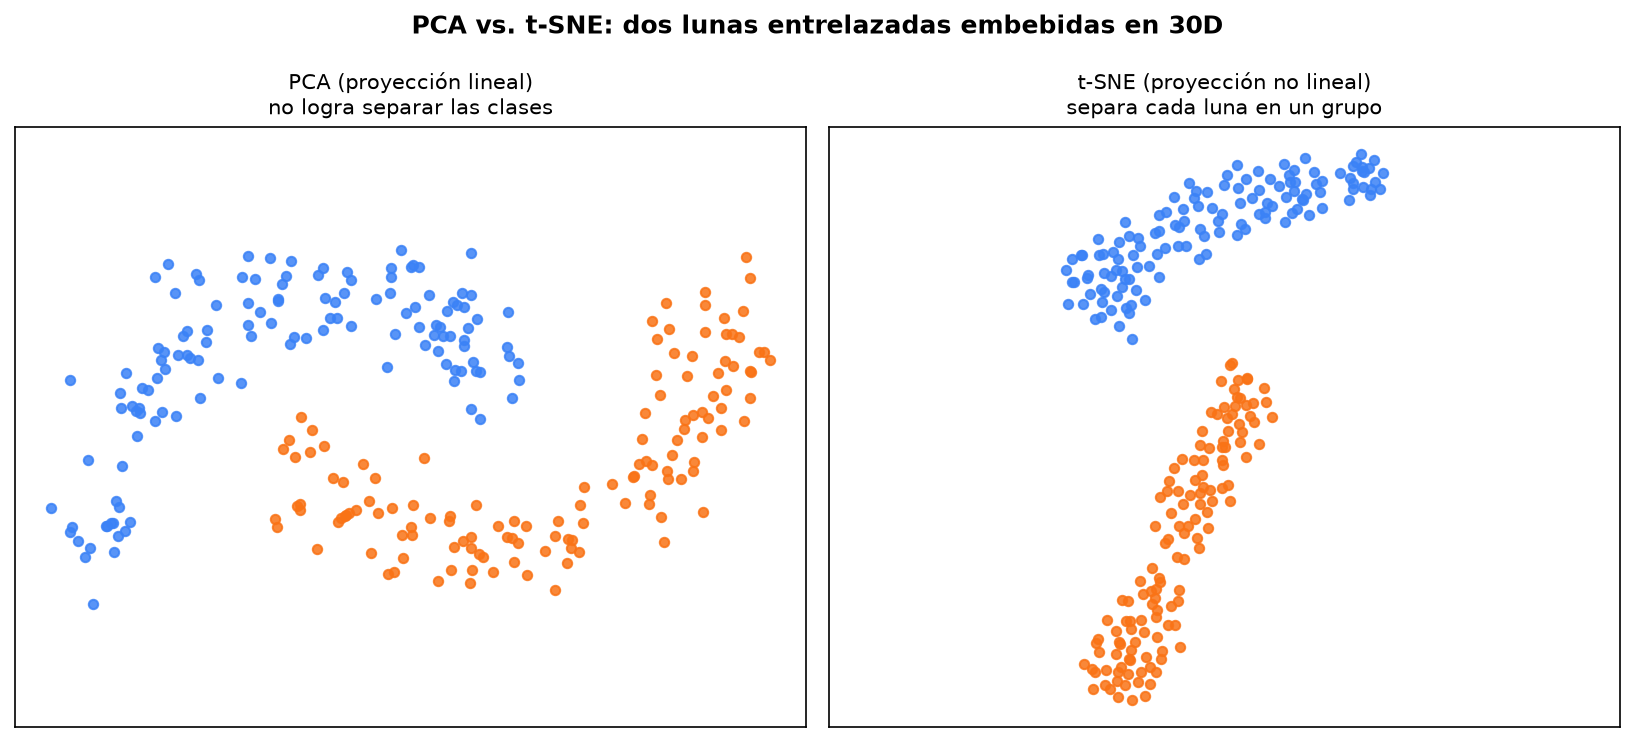
\includegraphics[width=0.68\textwidth]{../book/_static/generated/figures/es/pca_vs_tsne.png}
  \end{center}
\end{frame}

\begin{frame}{UMAP: rápido y preciso}
  \small
  UMAP es una de las técnicas de \textit{manifold learning} más potentes de la actualidad. A diferencia de $t$-SNE, que se centra casi exclusivamente en preservar vecindades muy locales, UMAP es capaz de preservar tanto la estructura \textbf{local} como la \textbf{global} de los datos, y además se ejecuta mucho más rápido sobre conjuntos de datos masivos, con millones de muestras.
  \begin{center}
    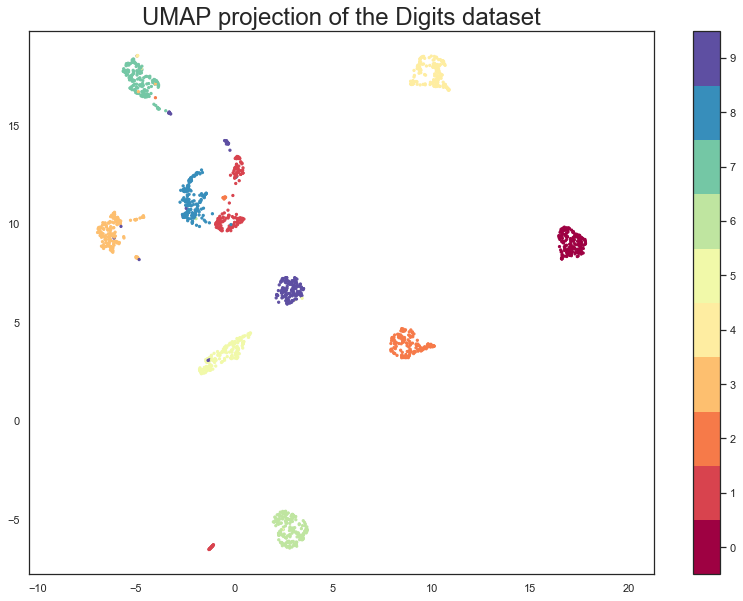
\includegraphics[width=0.36\textwidth]{../book/_static/external_images/umap_digits_projection.png}
  \end{center}
  \fuente{umap-learn docs, Copyright (c) 2017 Leland McInnes, licencia BSD-3.}
\end{frame}

% ============================================================
\section{3.3 Detección de anomalías}

\begin{frame}{Filosofía de la detección de anomalías}
  \small
  La detección de anomalías es una tarea no supervisada de gran relevancia industrial: identificar patrones inusuales o eventos sospechosos dentro de un flujo de datos. Se aplica en la detección de fraudes financieros, la prevención de intrusiones en redes, el control de calidad en fabricación y la limpieza automática de conjuntos de datos.

  A nivel conceptual, se basa en que los comportamientos normales (\textit{inliers}) son muy frecuentes y consistentes, mientras que las anomalías (\textit{outliers}) son eventos raros que se desvían significativamente de la norma. Se distinguen dos escenarios según la ``limpieza'' de los datos de entrenamiento:
  \begin{itemize}
    \item \textbf{\textit{Anomaly detection}}: el conjunto de entrenamiento puede contener ruido u \textit{outliers} sin depurar.
    \item \textbf{\textit{Novelty detection}}: el conjunto de entrenamiento está completamente limpio; el objetivo es detectar patrones nuevos nunca vistos.
  \end{itemize}
  \ejemplo{fraude bancario, fallos en una línea de producción, o un sensor que empieza a dar lecturas extrañas: en ninguno de estos casos sabemos de antemano cómo será la próxima anomalía, por eso se aborda como un problema no supervisado.}
\end{frame}

\begin{frame}{Enfoque gaussiano}
  \small
  Se asume que las observaciones normales se concentran en regiones del espacio de características con \textbf{alta densidad de probabilidad}. Se ajusta una distribución gaussiana a los datos normales, y cualquier punto con una densidad de probabilidad por debajo de un umbral se marca como anomalía. El umbral puede fijarse, por ejemplo, a partir de la tasa histórica conocida de casos raros (un 4\% de productos defectuosos, digamos).
  \begin{center}
    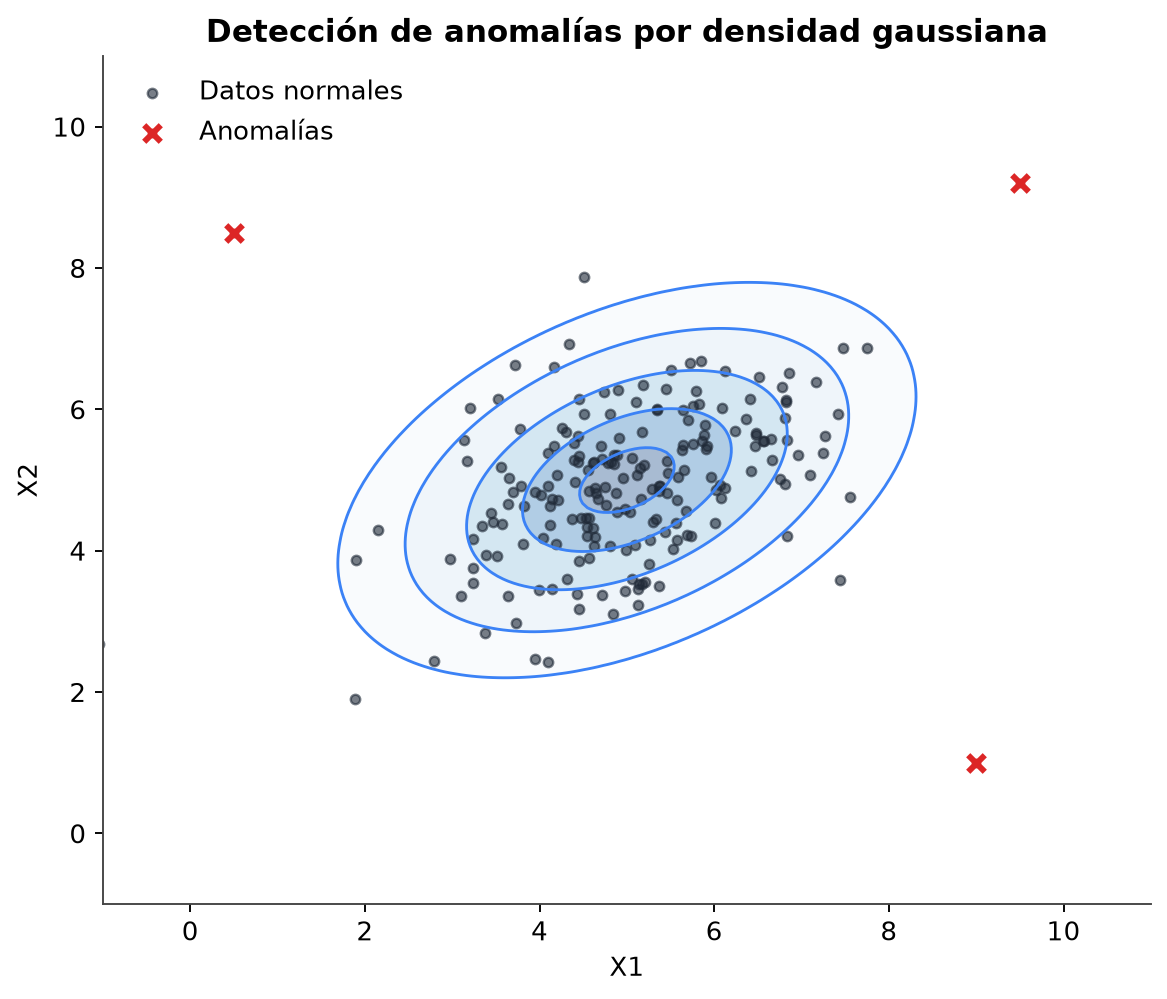
\includegraphics[width=0.36\textwidth]{../book/_static/generated/figures/es/gaussian_anomaly_detection.png}
  \end{center}
\end{frame}

\begin{frame}{Enfoque de reconstrucción con PCA}
  Esta técnica se basa en que los componentes principales mayoritarios de PCA capturan las direcciones que caracterizan el comportamiento \textbf{normal} del sistema. Se proyectan los datos a baja dimensión con PCA y se reconstruyen de vuelta al espacio original: como las componentes principales no capturan las desviaciones inusuales, las anomalías presentarán un \textbf{error de reconstrucción} mucho mayor que las instancias normales.
  \begin{center}
    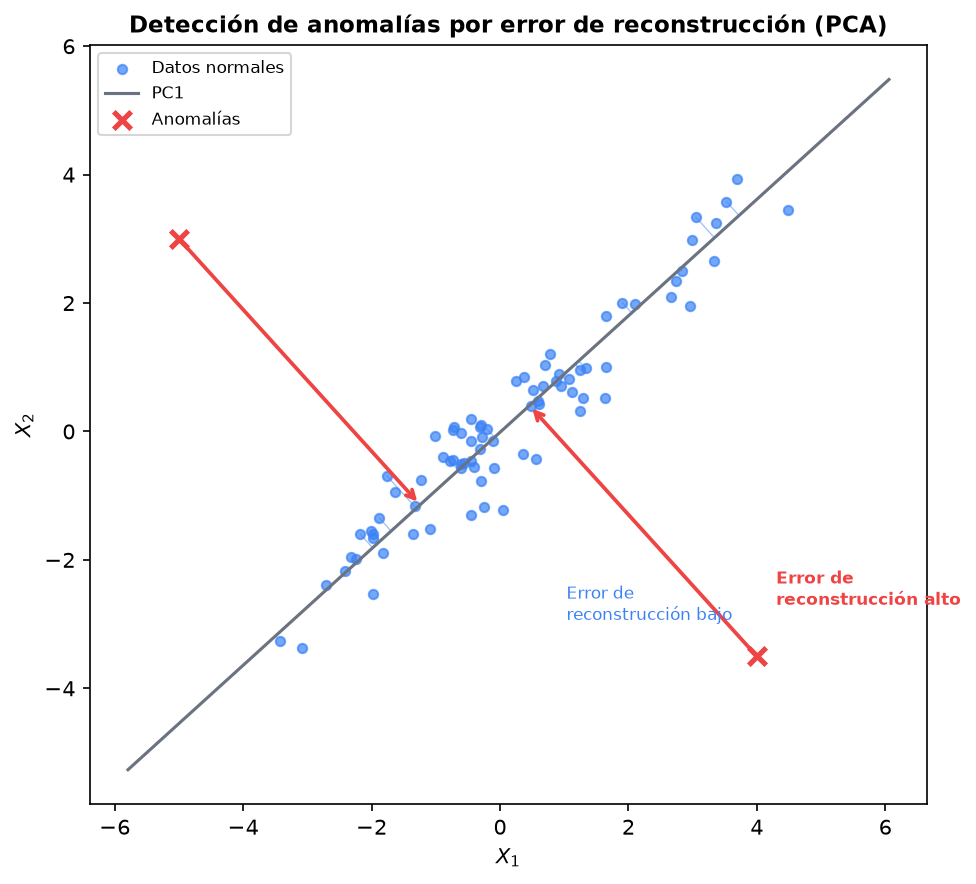
\includegraphics[width=0.36\textwidth]{../book/_static/generated/figures/es/pca_reconstruction_anomaly.png}
  \end{center}
\end{frame}

\begin{frame}{\textit{Isolation Forest}}
  \small
  A diferencia de los métodos anteriores, que modelan la densidad de los datos normales, \textbf{\textit{Isolation Forest}} busca \textbf{aislar} directamente cada observación mediante particiones aleatorias: en cada nodo de un árbol se elige al azar una característica y un umbral de corte, dividiendo los datos en dos.

  La intuición es simple: las anomalías, al estar alejadas del resto, requieren \textbf{muy pocas particiones} para quedar aisladas en su propia hoja, mientras que un punto normal necesita muchas más divisiones.
  \begin{center}
    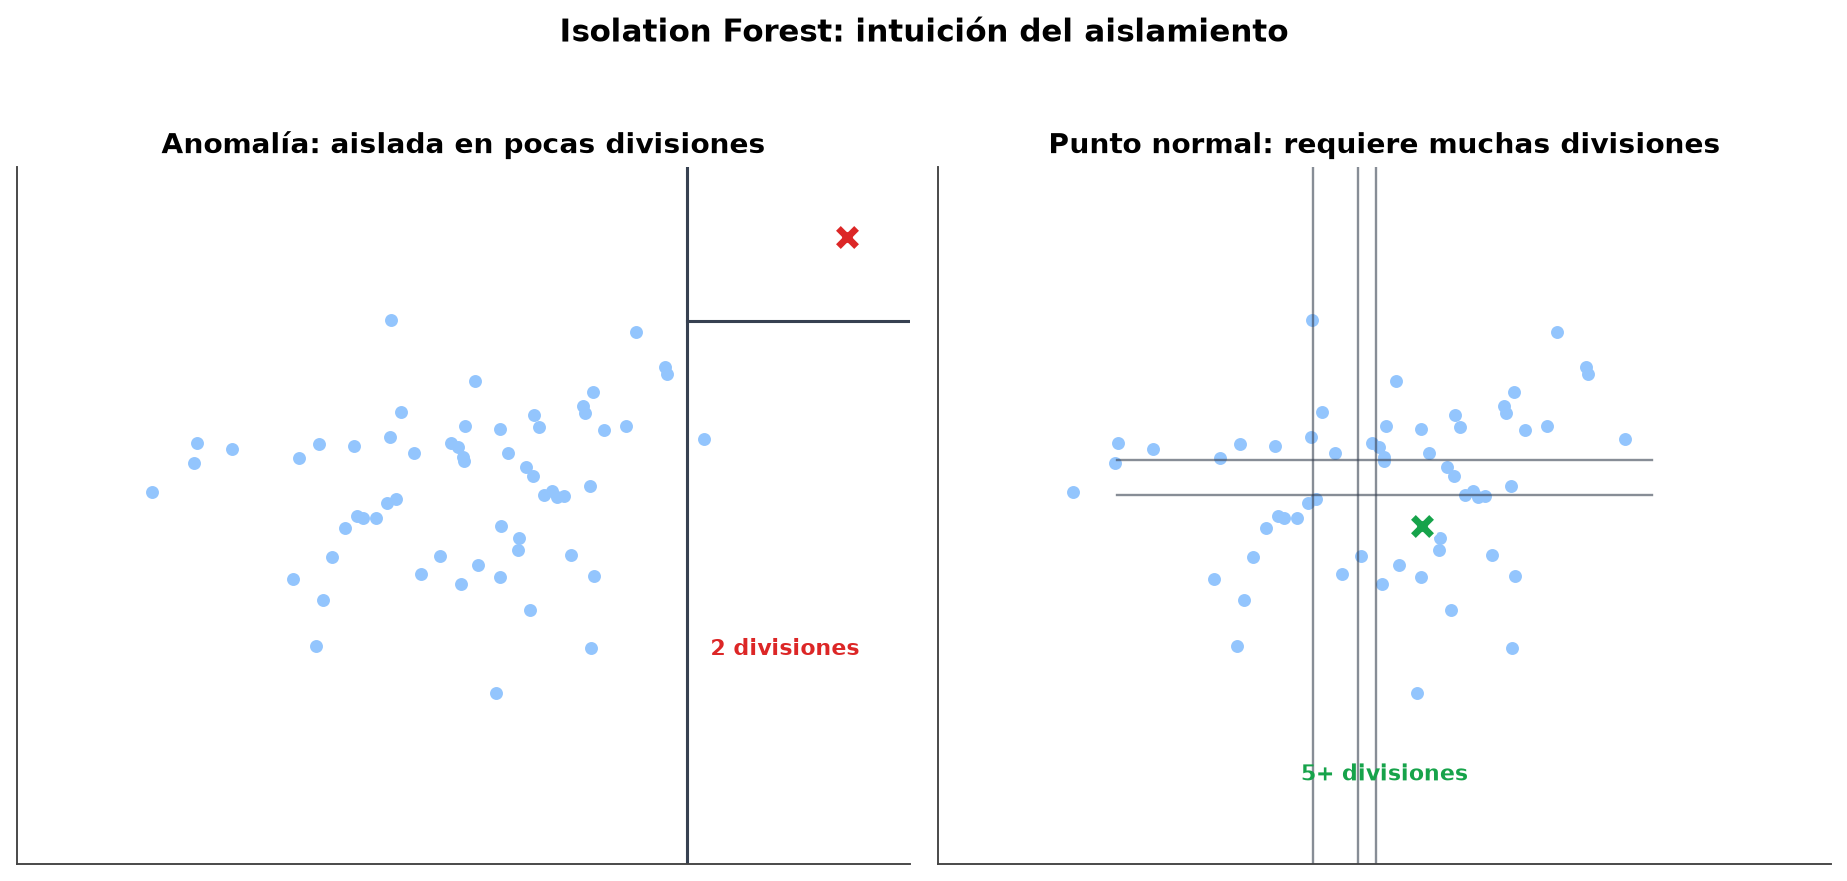
\includegraphics[width=0.68\textwidth]{../book/_static/generated/figures/es/isolation_forest_concept.png}
  \end{center}
\end{frame}

\begin{frame}{\textit{Local Outlier Factor} (LOF)}
  \small
  LOF compara la \textbf{densidad local} de una muestra con la de sus vecinos más cercanos. Una instancia normal tiene una densidad similar a su entorno; un \textit{outlier local} presenta una densidad mucho menor que sus vecinos inmediatos.

  Este método es muy útil para detectar \textbf{anomalías locales} que no destacarían en un análisis global, porque sus valores absolutos no son extremos, pero sí resultan inusuales dentro de su vecindario específico.
  \ejemplo{\footnotesize una casa de 200 m\textsuperscript{2} no es rara a nivel nacional, pero sí lo es en un barrio donde todas las casas miden 60 m\textsuperscript{2}: eso es lo que detecta LOF.}
  \begin{center}
    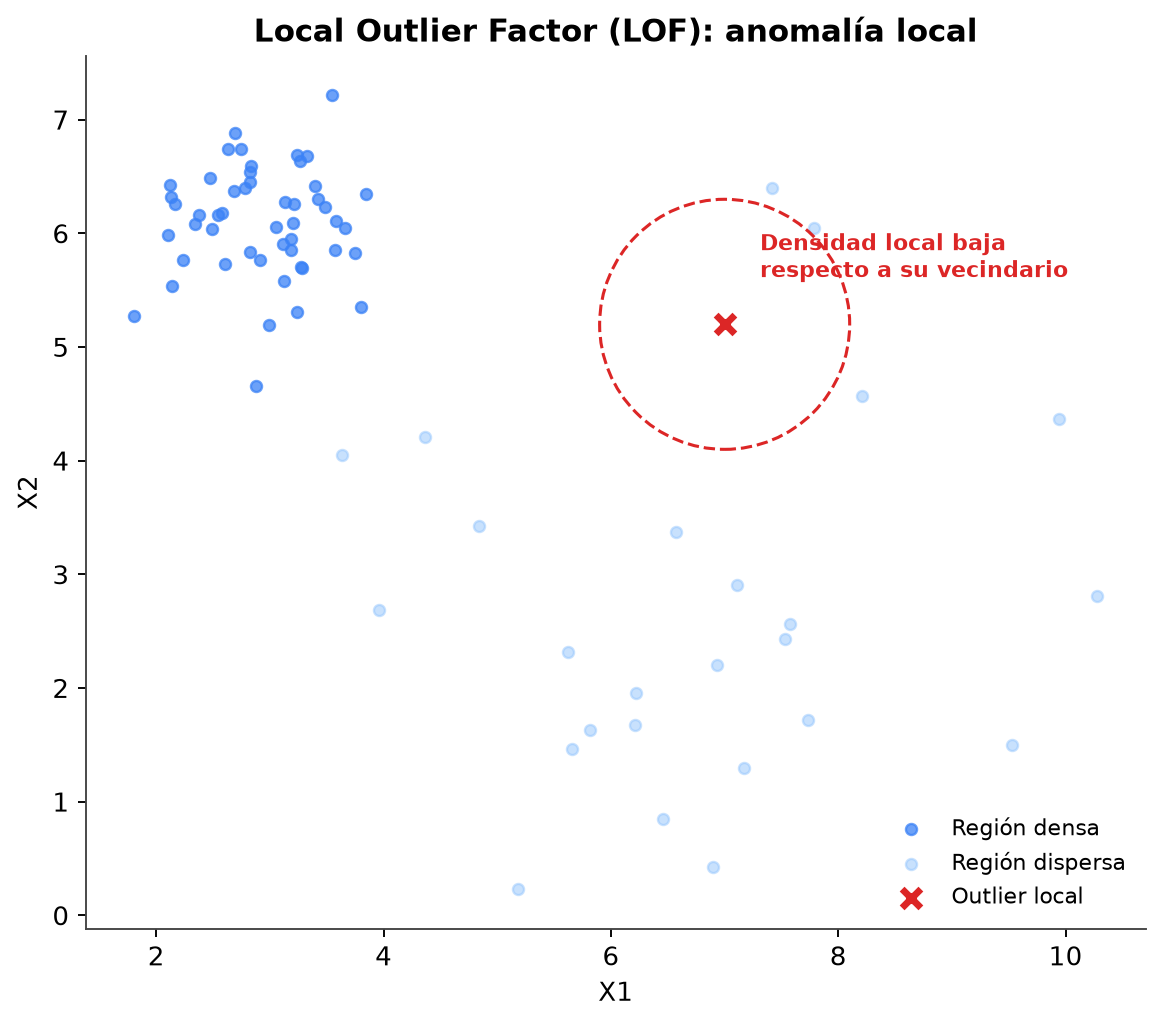
\includegraphics[width=0.26\textwidth]{../book/_static/generated/figures/es/lof_concept.png}
  \end{center}
\end{frame}

\begin{frame}{\textit{One-class} SVM}
  \small
  Este algoritmo está optimizado para \textit{novelty detection}, cuando se dispone de un conjunto de datos limpio para entrenar. En lugar de buscar un hiperplano que separe dos clases, proyecta los datos a un espacio de alta dimensión mediante un \textit{kernel} y busca la región de \textbf{volumen mínimo} que encierra casi todas las muestras de entrenamiento.

  Cualquier observación nueva que caiga fuera de esa región delimitada se clasifica automáticamente como anomalía o novedad.
  \begin{center}
    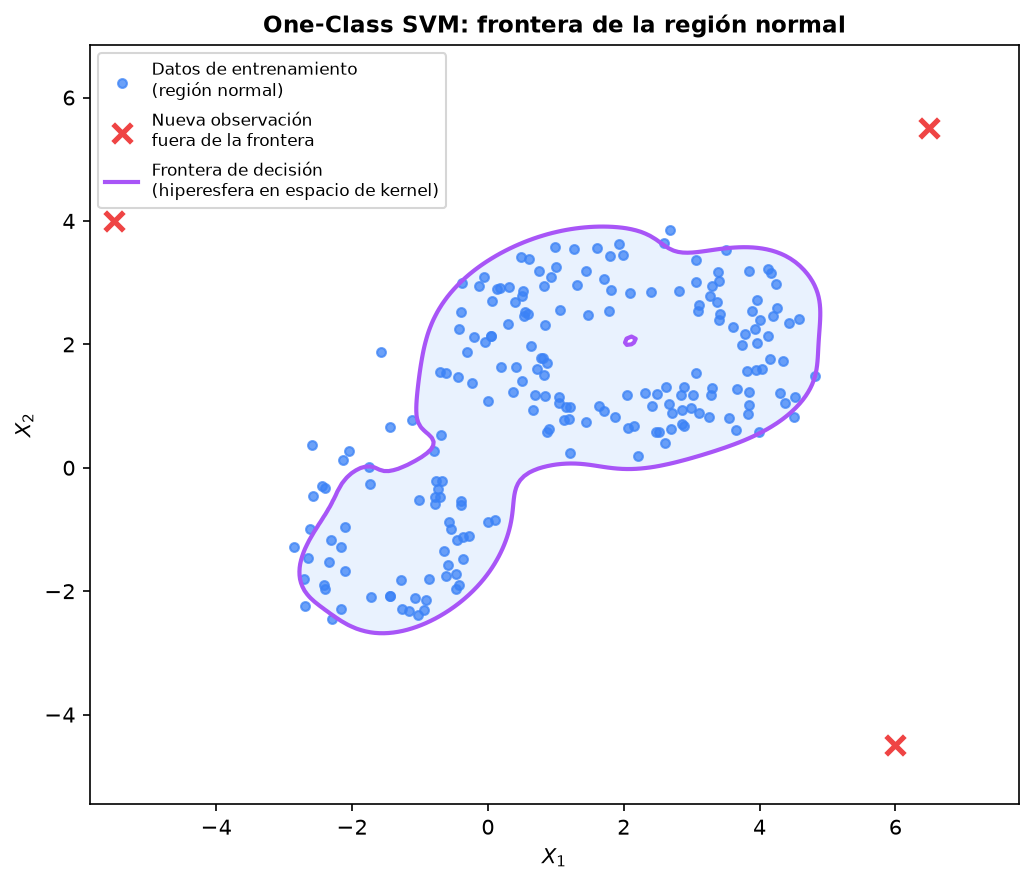
\includegraphics[width=0.34\textwidth]{../book/_static/generated/figures/es/one_class_svm_boundary.png}
  \end{center}
\end{frame}

% ============================================================
\begin{frame}{Resumen del capítulo}
  \small
  \begin{itemize}
    \item El aprendizaje no supervisado trabaja \textbf{sin etiquetas}, descubriendo la estructura latente de los propios datos.
    \item \textbf{$K$-\textit{means}} agrupa por centroides (rápido, requiere $K$ conocido); el \textbf{jerárquico} no necesita $K$ y ofrece un dendrograma visual; \textbf{DBSCAN} detecta formas arbitrarias y aísla el ruido.
    \item El \textbf{coeficiente de silueta} y el \textbf{estadístico \textit{gap}} son las herramientas más habituales para evaluar un \textit{clustering} sin etiquetas.
    \item La \textbf{maldición de la dimensionalidad} motiva reducir el número de variables antes de analizar o visualizar datos.
    \item \textbf{PCA} es rápido y lineal; \textbf{\textit{kernel} PCA}, \textbf{$t$-SNE} y \textbf{UMAP} capturan estructuras no lineales, con distintos equilibrios entre velocidad y fidelidad.
    \item La detección de \textbf{anomalías} combina enfoques estadísticos (gaussiano, reconstrucción con PCA) y algoritmos específicos (\textit{Isolation Forest}, LOF, \textit{one-class} SVM).
  \end{itemize}
\end{frame}

\titleslide

\end{document}
